\documentclass[letterpaper,addpoints,answers]{exam}
\usepackage{graphicx}
\usepackage{multicol}
\usepackage{tikz}

\makeatletter
\def\grd@save@target#1{%
  \def\grd@target{#1}}
\def\grd@save@start#1{%
  \def\grd@start{#1}}
\tikzset{
  grid with coordinates/.style={
    to path={%
      \pgfextra{%
        \edef\grd@@target{(\tikztotarget)}%
        \tikz@scan@one@point\grd@save@target\grd@@target\relax
        \edef\grd@@start{(\tikztostart)}%
        \tikz@scan@one@point\grd@save@start\grd@@start\relax
        \draw[minor help lines] (\tikztostart) grid (\tikztotarget);
        \draw[major help lines] (\tikztostart) grid (\tikztotarget);
        \grd@start
        \pgfmathsetmacro{\grd@xa}{\the\pgf@x/1cm}
        \pgfmathsetmacro{\grd@ya}{\the\pgf@y/1cm}
        \grd@target
        \pgfmathsetmacro{\grd@xb}{\the\pgf@x/1cm}
        \pgfmathsetmacro{\grd@yb}{\the\pgf@y/1cm}
        \pgfmathsetmacro{\grd@xc}{\grd@xa + \pgfkeysvalueof{/tikz/grid with coordinates/major step x}}
        \pgfmathsetmacro{\grd@yc}{\grd@ya + \pgfkeysvalueof{/tikz/grid with coordinates/major step y}}
        \foreach \x in {\grd@xa,\grd@xc,...,\grd@xb}
        \node[anchor=north] at (\x,\grd@ya) {\pgfmathprintnumber{\x}};
        \foreach \y in {\grd@ya,\grd@yc,...,\grd@yb}
        \node[anchor=east] at (\grd@xa,\y) {\pgfmathprintnumber{\y}};
      }
    }
  },
  minor help lines/.style={
    help lines,
    gray,
    line cap =round,
    xstep=\pgfkeysvalueof{/tikz/grid with coordinates/minor step x},
    ystep=\pgfkeysvalueof{/tikz/grid with coordinates/minor step y}
  },
  major help lines/.style={
    help lines,
    line cap =round,
    line width=\pgfkeysvalueof{/tikz/grid with coordinates/major line width},
    xstep=\pgfkeysvalueof{/tikz/grid with coordinates/major step x},
    ystep=\pgfkeysvalueof{/tikz/grid with coordinates/major step y}
  },
  grid with coordinates/.cd,
  minor step x/.initial=.5,
  minor step y/.initial=.2,
  major step x/.initial=1,
  major step y/.initial=1,
  major line width/.initial=1pt,
}
\makeatother


\begin{document}

\begin{coverpages}
 \large\bfseries
 
 \noindent 
 Physics 107: Physics for Life-Sciences

 \vspace{2ex}
 \noindent
 Midterm Exam: September 22, 2014

 \vspace{3ex}
 \noindent 
 This test is administered under the rules and regulations of the honor code of the College of William \& Mary.

 \vspace{2ex}
 \noindent 
 Name:\enspace\makebox[2.3in]{\hrulefill} \\

 \noindent 
 Signature:\enspace\makebox[2in]{\hrulefill} \\

 \vspace{5ex}
 \noindent 
 Instructions:
 \begin{itemize}
  \item This is a closed book, closed notes test.
  \item Calculators are permitted, but not laptops or cell phones. Devices with wireless connections are not allowed.
  \item Start your work from the fundamental equations on the formula sheet, and derive any additional expressions that you may need.
  \item Circle your answer for each part of each problem. 
  \item Clearly mark out any work that you wish the grader to disregard.  Do not waste your time erasing.
  \item Your work will be graded based on your ability to write down a logical and organized solution grounded in the correct assessment of the physics of a situation. No credit will be given for an answer that is not justified by a logical solution or where that justification is not organized or readable. Partial credit will be given up to the point where your solution departs from a correct analysis of the physics involved for any given part of a problem.
 \end{itemize}

 \pagebreak

 \begin{center}
  \gradetable[v][questions]
 \end{center}
 
\end{coverpages}
 

\begin{questions}

\question
You are operating a small remote controlled toy car on the sidewalk along Jamestown Road. As you are standing on the sidewalk, the speed of the toy car relative to you is plotted below.
\begin{center}
 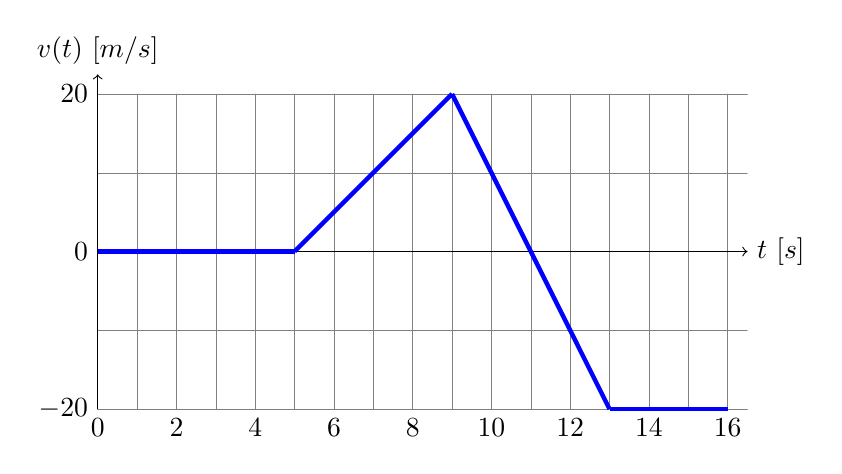
\begin{tikzpicture}[xscale=0.5,yscale=0.1,grid with coordinates/major step x=2,grid with coordinates/minor step x=1,grid with coordinates/major step y=20,grid with coordinates/minor step y=10,grid with coordinates/major line width=0.2pt]
  \draw (0,-20) to[grid with coordinates] (16.5,20);
  \draw[->] (0,0) -- (16.5,0) node[right] {$t~[s]$};
  \draw[->] (0,-20) -- (0,22.5) node[above] {$v(t)~[m/s]$};
  \draw[ultra thick,color=blue] (0.0,0.0) -- (5.0,0.0);
  \draw[ultra thick,color=blue] (5.0,0.0) -- (9.0,20.0);
  \draw[ultra thick,color=blue] (9.0,20.0) -- (13.0,-20.0);
  \draw[ultra thick,color=blue] (13.0,-20.0) -- (16.0,-20.0);
 \end{tikzpicture}
\end{center}

\begin{parts}
 \part[5]
  What is the acceleration $\vec{a}_1$ between $t = 5$\,s and $t = 9$\,s, and what is the acceleration $\vec{a}_2$ between $t = 9$\,s and $t = 13$\,s?
  \vspace{6\baselineskip}
 \part[15]
  Assuming the car started at $x = 0$\,m, plot the position versus time. Mark in particular the position at $t = 5$\,s, $t = 9$\,s, and $t = 13$\,s. Use the back of this page for any calculations.
  \begin{center}
   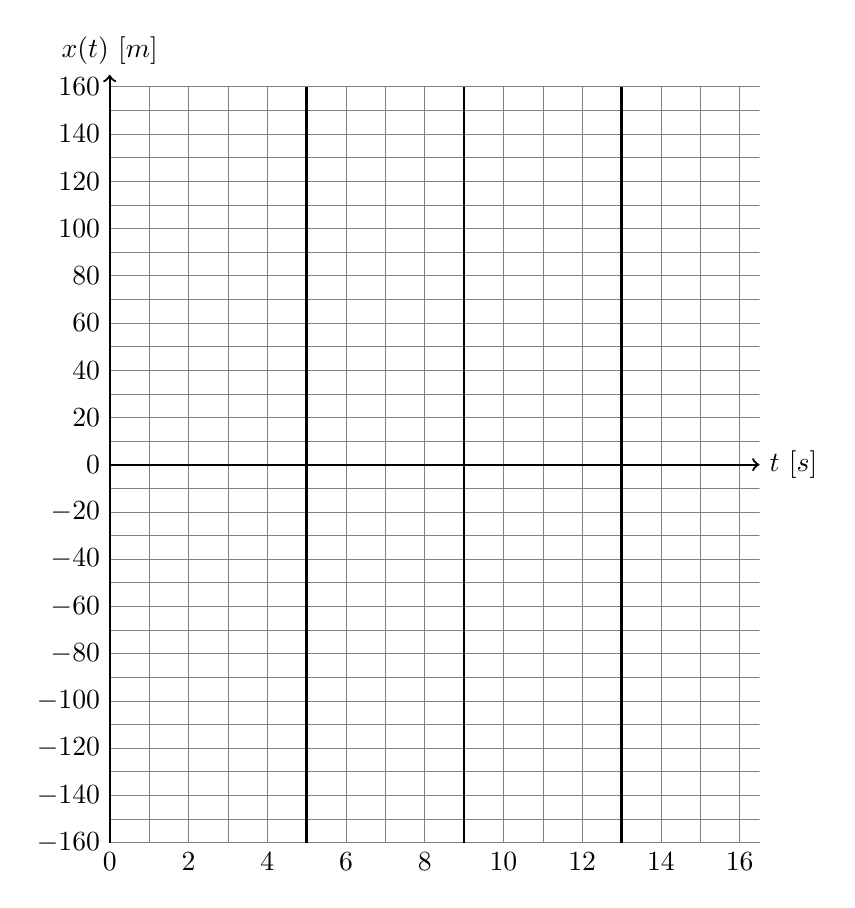
\begin{tikzpicture}[xscale=0.5,yscale=0.03,grid with coordinates/major step x=2,grid with coordinates/minor step x=1,grid with coordinates/major step y=20,grid with coordinates/minor step y=10,grid with coordinates/major line width=0.2pt]
    \draw (0,-160) to[grid with coordinates] (16.5,160);
    \draw[thick] (5,-160) -- (5,160);
    \draw[thick] (9,-160) -- (9,160);
    \draw[thick] (13,-160) -- (13,160);
    \draw[thick,->] (0,0) -- (16.5,0) node[right] {$t~[s]$};
    \draw[thick,->] (0,-160) -- (0,165) node[above] {$x(t)~[m]$};
   \end{tikzpicture}
  \end{center}
\end{parts}

\pagebreak

\question

To celebrate her good performance on a physics test, Alice decides to break out a bottle of champaign.  In order to avoid property damage, she takes the bottle outside to uncork it.  The cork pops off the champaign bottle with a velocity of 20.0\,m/s at an angle of $30^\circ$ relative to the vertical.  When the cork is released, Alice is holding the bottle such that the cork is 1.50\,m above the ground.
\begin{parts}
 \part[5]
  Draw a diagram of this situation.  Indicate the direction of any relevant vectors and coordinate systems.
  \vspace{10\baselineskip}
 \part[5]
  What is the maximum height above the ground that the cork reaches?
  \vspace{10\baselineskip}
 \part[5]
  How long does it take before the cork touches the ground?
  \vspace{14\baselineskip}
 \part[5]
  How far does Alice have to walk to retrieve the cork?
  \vspace{6\baselineskip}
\end{parts}

\pagebreak

\question
You are holding out your stretched arm horizontally with a physics textbook of 2\,kg in your hand; your entire arm itself has a mass of 10\,kg. Your deltoid muscle, which connects the scapula (shoulder blade) to the humerus (upper arm), provides the force necessary to hold up your arm with the book in your hand.\footnotemark{} The angle between the humerus and the deltoid is $20^\circ$.

\emph{Note:} Remember to consider the horizontal force $\vec{N}$ that the scapula is providing against the humerus. 

\footnotetext{For this problem we are ignoring the supraspinatus muscle since it is mostly effective when the arm is nearer to the body.}

\begin{center}
 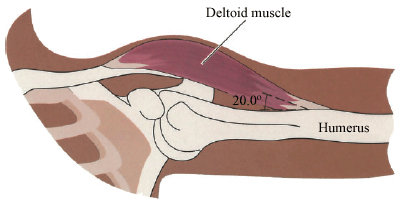
\includegraphics[width=0.4\textwidth]{test1/humerus-deltoid}
\end{center}

\begin{parts}
 \part[5]
  Draw the free-body diagram for your arm and all of the forces working on it.
  \vspace{10\baselineskip}
 \part[5]
  Write down the components of the force vectors in a coordinate system of your choice.
  \vspace{10\baselineskip}
 \part[10]
  Using Newton's 1st law, find the tension $T$ in the deltoid muscle.
  \vspace{12\baselineskip}
\end{parts}


\pagebreak

\question
A ``turnpike double'' (TPD) is a specific configuration of a tractor-trailer where the tractor unit pulls two trailers with a length of up to 48\,ft each (the size of a shipping container). In this problem we consider a FedEx tractor-trailer where the two trailers have a total mass of $M_1 = M_2 = 25\,000$\,kg each and the tractor unit has a total mass of $M_0 = 10\,000$\,kg. The entire tractor-trailer departs from rest with an acceleration of 1\,m/s$^2$. Denote the tension in the coupling between the tractor unit and the first trailer as $T_0$ and the tension in the coupling between the two trailers as $T_{12}$.

\emph{Note:} Assume that only the tractor unit is affected by friction. You do not need to use any coefficients of friction for this problem. You only need Newton's laws of motion for this problem.
\begin{center}
 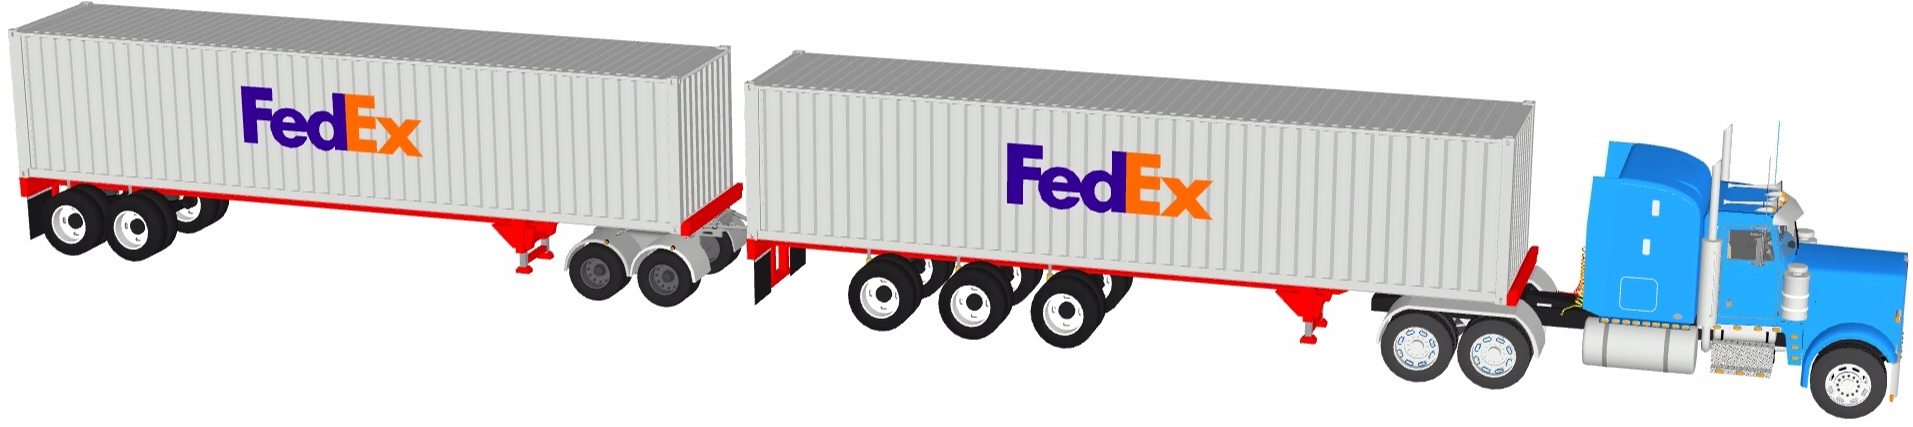
\includegraphics[width=0.9\textwidth]{test1/tpd}
\end{center}

\begin{parts}
 \part[10]
  Draw the free-body diagrams for each of the trailers and for the tractor unit (\textit{i.e.} three diagrams). Consider both horizontal and vertical forces.
  \vspace{12\baselineskip}
 \part[5]
  Considering the entire tractor-trailer as a single system, what is the magnitude of the force of friction that the ground exerts on the wheels of the tractor unit?
  \vspace{10\baselineskip}
 \part[5]
  Considering the components as separate systems, what is the tension $T_{12}$ in the coupling between the two trailers?
  \vspace{10\baselineskip}
\end{parts}



\end{questions}

 \pagebreak
 
 {\Large Possibly useful relations (feel free to detach this page):}
  
 \fontseries{\seriesdefault}
 \begin{multicols}{2}
 \Large
 \noindent
 $\vec{v}_{avg} = \Delta\vec{x} / \Delta t$ \\
 $x = x_0 + v_0 t + \frac{1}{2} a t^2$ \\
 $v^2 = v_0^2 + 2 a (x - x_0)$ \\
 $R = \frac{v_0^2}{g}\sin 2\theta$ \\
 $\vec{F}_{net} = m \vec{a}$ \\
 $\vec{W} = m \vec{g}$ \\
 $\vec{g} = 9.80\,m/s^2$ downward \\
 $\cos\theta = \hbox{adjacent}/\hbox{hypotenuse}$ \\
 $\sin\theta = \hbox{opposite}/\hbox{hypotenuse}$ \\
 
 \noindent
 $\vec{a}_{avg} = \Delta\vec{v} / \Delta t$ \\
 $v = v_0 + a t$ \\
 $v_{avg} = \frac{v_0 + v}{2}$ \\
 $h = \frac{v_0^2}{2 g} \sin^2 \theta$ \\
 $\vec{F}_{BA} = - \vec{F}_{AB}$ \\
 $0 \le f_s \le \mu_s N$ \\
 $f_k = \mu_k N$ \\
 $\tan\theta = \sin\theta / \cos\theta$ \\
 $x = \frac{-b \pm \sqrt{b^2 - 4 a c}}{2 a}$ \\
 \end{multicols}

\end{document}
